\documentclass{standalone}
% \usepackage[french]{babel}
% \selectlanguage{french}
\usepackage[T1]{fontenc}
\usepackage[utf8]{inputenc}
\usepackage{lmodern}
\usepackage{pgfplots}
\usepackage{tikz}
\begin{document}
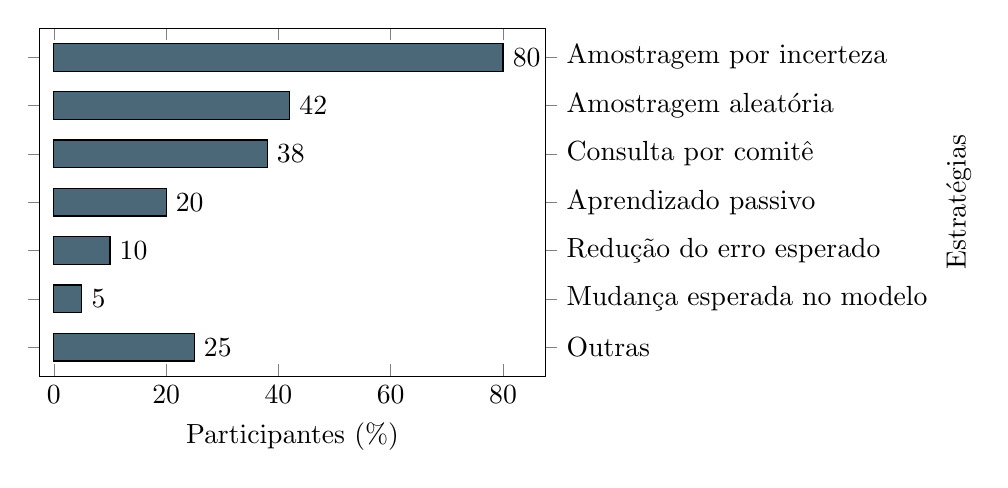
\begin{tikzpicture}
\begin{axis}[
    xbar, width=8cm, height=6cm,
%     y=1cm, bar width=0.9cm,
%     xmin=0.0,
%     width=12cm,
%     height=40cm,
%     enlarge x limits={rel=0.13,upper},
	ylabel near ticks, yticklabel pos=right,
    ytick={1,2,3,4,5,6,7},
    yticklabels={
    {Amostragem por incerteza},
    {Amostragem aleatória},
    {Consulta por comitê},
    {Aprendizado passivo},
    {Redução do erro esperado},
    {Mudança esperada no modelo},
    {Outras}
    },
%         enlarge y limits=0.4,
    xlabel={Participantes (\%)},
    ylabel=Estratégias,
    ytick=data,
    nodes near coords,
    nodes near coords align=horizontal
]
\addplot [draw=black, fill=cyan!40!black] coordinates {
    (80,7)
    (42,6)
    (38,5)
    (20,4)
    (10,3)
    (5,2)
    (25,1)
};
\end{axis}
\end{tikzpicture}
\end{document}